\documentclass[12pt,spanish,fleqn,openany,letterpaper,pagesize]{scrbook}

\usepackage{times}
%\usepackage[ansinew]{inputenc}
\usepackage[spanish]{babel}
\usepackage{fancyhdr}
\usepackage{epsfig}
\usepackage{epic}
\usepackage{eepic}
\usepackage{amsmath}
\usepackage{threeparttable}
\usepackage{amscd}
\usepackage{here}
\usepackage{graphicx}
\usepackage{lscape}
\usepackage{tabularx}
\usepackage{subfigure}
\usepackage{longtable}
\usepackage[usenames]{color}


\usepackage{rotating} %Para rotar texto, objetos y tablas seite. No se ve en DVI solo en PS. Seite 328 Hundebuch
                        %se usa junto con \rotate, \sidewidestable ....


\renewcommand{\theequation}{\thechapter-\arabic{equation}}
\renewcommand{\thefigure}{\textbf{\thechapter-\arabic{figure}}}
\renewcommand{\thetable}{\textbf{\thechapter-\arabic{table}}}


\pagestyle{fancyplain}%\addtolength{\headwidth}{\marginparwidth}
\textheight22.5cm \topmargin0cm \textwidth16.5cm
\oddsidemargin0.5cm \evensidemargin-0.5cm%
\renewcommand{\chaptermark}[1]{\markboth{\thechapter\; #1}{}}
\renewcommand{\sectionmark}[1]{\markright{\thesection\; #1}}
\lhead[\fancyplain{}{\thepage}]{\fancyplain{}{\rightmark}}
\rhead[\fancyplain{}{\leftmark}]{\fancyplain{}{\thepage}}
\fancyfoot{}
\thispagestyle{fancy}%


\addtolength{\headwidth}{0cm}
\unitlength1mm %Define la unidad LE para Figuras
\mathindent0cm %Define la distancia de las formulas al texto,  fleqn las descentra
\marginparwidth0cm
\parindent0cm %Define la distancia de la primera linea de un parrafo a la margen

%Para tablas,  redefine el backschlash en tablas donde se define la posici\'{o}n del texto en las
%casillas (con \centering \raggedright o \raggedleft)
\newcommand{\PreserveBackslash}[1]{\let\temp=\\#1\let\\=\temp}
\let\PBS=\PreserveBackslash

%Espacio entre lineas
\renewcommand{\baselinestretch}{1.1}

%Neuer Befehl f\"{u}r die Tabelle Eigenschaften der Aktivkohlen
\newcommand{\arr}[1]{\raisebox{1.5ex}[0cm][0cm]{#1}}

%Neue Kommandos
\usepackage{Befehle}

\graphicspath{{/home/franklin/Documentos/GitHub/TDG/Scripts/Plots/}} %Setting the graphicspath

\setlength{\parskip}{1em}


%Trennungsliste
\hyphenation {Reaktor-ab-me-ssun-gen Gas-zu-sa-mmen-set-zung
Raum-gesch-win-dig-keit Durch-fluss Stick-stoff-gemisch
Ad-sorp-tions-tem-pe-ra-tur Klein-schmidt
Kohlen-stoff-Mole-kular-siebe Py-rolysat-aus-beu-te
Trans-port-vor-gan-ge}
%\includeonly{Kap1/Kap1,Kap2/Kap2}
\begin{document}
\pagenumbering{roman}
%\newpage
%\setcounter{page}{1}
\begin{center}
\begin{figure}
\centering%

\epsfig{file=HojaTitulo/EscudoUN-cropped.pdf,scale=1}%
\end{figure}
\thispagestyle{empty} \vspace*{2.0cm} \textbf{\huge
T\'{\i}tulo de la tesis  o trabajo de investigaci\'{o}n}\\[6.0cm]
\Large\textbf{Franklin Farid Ayala Cruz}\\[6.0cm]
\small Universidad Nacional de Colombia\\
Facultad de Minas, Departamento de Ingenier\'{i}a Civil\\
Medell\'{i}n, Colombia\\
2020\\
\end{center}

\newpage{\pagestyle{empty}\cleardoublepage}

\newpage
\begin{center}
\thispagestyle{empty} \vspace*{0cm} \textbf{\huge
T\'{\i}tulo de la tesis  o trabajo de investigaci\'{o}n}\\[3.0cm]
\Large\textbf{Franklin Farid Ayala Cruz}\\[3.0cm]
\small Tesis o trabajo de grado presentada(o) como requisito parcial para optar al
t\'{\i}tulo de:\\
\textbf{Ingeniero Civil}\\[2.5cm]
Director(a):\\
T\'{\i}tulo (Ph.D., Doctor, Qu\'{\i}mico, etc.) y Andrés Fernando Osorio Arias\\[2.0cm]
L\'{\i}nea de Investigaci\'{o}n:\\
Oceanograf\'{i}a e ingenier\'{i}a costera\\
Grupo de Investigaci\'{o}n:\\
OCE\'{A}NICOS\\[2.5cm]
Universidad Nacional de Colombia\\
Facultad de Minas, Departamento de Geociencias y Medio Ambiente\\
Medell\'{i}n, Colombia\\
2020\\
\end{center}

\newpage{\pagestyle{empty}\cleardoublepage}

\newpage
\thispagestyle{empty} \textbf{}\normalsize
\\\\\\%
\textbf{(Dedicatoria o un lema)}\\[4.0cm]

\begin{flushright}
\begin{minipage}{8cm}
    \noindent
        \small
        Su uso es opcional y cada autor podr\'{a} determinar la distribuci\'{o}n del texto en la p\'{a}gina, se sugiere esta presentaci\'{o}n. En ella el autor dedica su trabajo en forma especial a personas y/o entidades.\\[1.0cm]\\
        Por ejemplo:\\[1.0cm]
        A mis padres\\[1.0cm]\\
        o\\[1.0cm]
        La preocupaci\'{o}n por el hombre y su destino siempre debe ser el
        inter\'{e}s primordial de todo esfuerzo t\'{e}cnico. Nunca olvides esto
        entre tus diagramas y ecuaciones.\\\\
        Albert Einstein\\
\end{minipage}
\end{flushright}

\newpage{\pagestyle{empty}\cleardoublepage}

\newpage
\thispagestyle{empty} \textbf{}\normalsize
\\\\\\%
\textbf{\LARGE Agradecimientos}
\addcontentsline{toc}{chapter}{\numberline{}Agradecimientos}\\\\
Esta secci\'{o}n es opcional, en ella el autor agradece a las personas o instituciones que colaboraron en la realizaci\'{o}n de la tesis  o trabajo de investigaci\'{o}n. Si se incluye esta secci\'{o}n, deben aparecer los nombres completos, los cargos y su aporte al documento.\\

\newpage{\pagestyle{empty}\cleardoublepage}

\newpage
\textbf{\LARGE Resumen}
\addcontentsline{toc}{chapter}{\numberline{}Resumen}\\\\
El resumen es una presentaci\'{o}n abreviada y precisa (la NTC 1486 de 2008 recomienda revisar la norma ISO 214 de 1976). Se debe usar una extensi\'{o}n m\'{a}xima de 12 renglones. Se recomienda que este resumen sea anal\'{\i}tico, es decir, que sea completo, con informaci\'{o}n cuantitativa y cualitativa, generalmente incluyendo los siguientes aspectos: objetivos, dise\~{n}o, lugar y circunstancias, pacientes (u objetivo del estudio), intervenci\'{o}n, mediciones y principales resultados, y conclusiones. Al final del resumen se deben usar palabras claves tomadas del texto (m\'{\i}nimo 3 y m\'{a}ximo 7 palabras), las cuales permiten la recuperaci\'{o}n de la informaci\'{o}n.\\

\textbf{\small Palabras clave: (m\'{a}ximo 10 palabras, preferiblemente seleccionadas de las listas internacionales que permitan el indizado cruzado)}.\\

A continuaci\'{o}n se presentan algunos ejemplos de tesauros que se pueden consultar para asignar las palabras clave, seg\'{u}n el \'{a}rea tem\'{a}tica:\\

\textbf{Artes}: AAT: Art y Architecture Thesaurus.

\textbf{Ciencias agropecuarias}: 1) Agrovoc: Multilingual Agricultural Thesaurus - F.A.O. y 2)GEMET: General Multilingual Environmental Thesaurus.

\textbf{Ciencias sociales y humanas}: 1) Tesauro de la UNESCO y 2) Population Multilingual Thesaurus.

\textbf{Ciencia y tecnolog\'{\i}a}: 1) Astronomy Thesaurus Index. 2) Life Sciences Thesaurus, 3) Subject Vocabulary, Chemical Abstracts Service y 4) InterWATER: Tesauro de IRC - Centro Internacional de Agua Potable y Saneamiento.

\textbf{Tecnolog\'{\i}as y ciencias m\'{e}dicas}: 1) MeSH: Medical Subject Headings (National Library of Medicine's USA) y 2) DECS: Descriptores en ciencias de la Salud (Biblioteca Regional de Medicina BIREME-OPS).

\textbf{Multidisciplinarias}: 1) LEMB - Listas de Encabezamientos de Materia y 2) LCSH- Library of Congress Subject Headings.\\

Tambi\'{e}n se pueden encontrar listas de temas y palabras claves, consultando las distintas bases de datos disponibles a trav\'{e}s del Portal del Sistema Nacional de Bibliotecas\footnote{ver: www.sinab.unal.edu.co}, en la secci\'{o}n "Recursos bibliogr\'{a}ficos" opci\'{o}n "Bases de datos".\\

\textbf{\LARGE Abstract}\\\\
Es el mismo resumen pero traducido al ingl\'{e}s. Se debe usar una extensi\'{o}n m\'{a}xima de 12 renglones. Al final del Abstract se deben traducir las anteriores palabras claves tomadas del texto (m\'{\i}nimo 3 y m\'{a}ximo 7 palabras), llamadas keywords. Es posible incluir el resumen en otro idioma diferente al espa\~{n}ol o al ingl\'{e}s, si se considera como importante dentro del tema tratado en la investigaci\'{o}n, por ejemplo: un trabajo dedicado a problemas ling\"{u}\'{\i}sticos del mandar\'{\i}n seguramente estar\'{\i}a mejor con un resumen en mandar\'{\i}n.\\[2.0cm]
\textbf{\small Keywords: palabras clave en ingl\'{e}s(m\'{a}ximo 10 palabras, preferiblemente seleccionadas de las listas internacionales que permitan el indizado cruzado)}\\

\renewcommand{\tablename}{\textbf{Tabla}}
\renewcommand{\figurename}{\textbf{Figura}}
\renewcommand{\listtablename}{Lista de Tablas}
\renewcommand{\listfigurename}{Lista de Figuras}
\renewcommand{\contentsname}{Contenido}


%\newcommand{\clearemptydoublepage}{\newpage{\pagestyle{empty}\cleardoublepage}}
\tableofcontents
\chapter*{Lista de s\'{\i}mbolos}
\addcontentsline{toc}{chapter}{\numberline{}Lista de s\'{\i}mbolos}
Esta secci\'{o}n es opcional, dado que existen disciplinas que no manejan s\'{\i}mbolos y/o abreviaturas.\\

Se incluyen s\'{\i}mbolos generales (con letras latinas y griegas), sub\'{\i}ndices, super\'{\i}ndices y abreviaturas (incluir s\'{o}lo las clases de s\'{\i}mbolos que se utilicen). Cada una de estas listas debe estar ubicada en orden alfab\'{e}tico de acuerdo con la primera letra del s\'{\i}mbolo.
\section*{S\'{\i}mbolos con letras latinas}
 \label{simbolos}
 \renewcommand{\arraystretch}{1.3}
%\begin{longtable}[l]{*{4}{>{$}l<{$}}p{9cm}}
\begin{longtable}[l]{>{$}l<{$}l>{$}l<{$}>{$}l<{$}}
%\begin{tabular}
\textbf{S\'{\i}mbolo}&\textbf{T\'{e}rmino}&\textbf{Unidad SI}&\textbf{Definici\'{o}n}\\[0.5ex]\hline
\endfirsthead%
\textbf{S\'{\i}mbolo}&\textbf{T\'{e}rmino}&\textbf{Unidad SI}&\textbf{Definici\'{o}n}\\[0.5ex]\hline
\endhead%
      A              &\'{A}rea                                   &\text{m}^{2}                         &\int\int dxdy\\%
      A_{\text{BET}} &\'{A}rea interna del s\'{o}lido                &\frac{\text{m}^{2}}{\text{g}}        &\text{ver DIN ISO 9277}\\%
      A_{\text{g}}   &\'{A}rea transversal de la fase gaseosa    &\text{m}^{2}                         &\text{Ec...}\\%
      A_{\text{s}}   &\'{A}rea transversal de la carga a granel  &\text{m}^{2}                         &\text{Ec...}\\%
      a              &Coeficiente                            &1                                    &\text{Ec...}\\%
      a              &Contenido de ceniza                    &1                                    &\frac{m_{\text{ceniza}}}{m_{\text{bm,0}}}\\%
      c              &Contenido de carbono                   &1                                    &\frac{m_{\text{C}}}{m}\\%
      c              &Longitud de la cuerda                  &\text{m}                             &\text{Figura...}\\
      c              &Concentraci\'{o}n de la cantidad de materia&\frac{\text{mol}}{\text{m}^{3}}      &\frac{n}{V}\\%
      D              &Di\'{a}metro                               &\text{m}                             &\\%
      E_{\text{A}}   &Energ\'{\i}a de activaci\'{o}n                  &\frac{\text{kJ}}{\text{mol}}         &\text{Ec....}\\%
      F              &Fracci\'{o}n de materia vol\'{a}til            &1                                    &\text{ver DIN 51720}\\%
      Fr             &N\'{u}mero de Froude                       &1                                    &\frac{\omega^{2}R}{g_{\text{0}}}\\%
      \overrightarrow{g}&Aceleraci\'{o}n de la gravedad          &\frac{\text{m}}{\text{s}^{2}}        &\frac{d^{2}\overrightarrow{r}}{dt^{2}}\\%
      H              &Entalp\'{\i}a                               &\text{J}                             &U+PV\\%
      H_{\text{o}}   &Poder calor\'{\i}fico superior              &\frac{\text{MJ}}{\text{kg}}          &\text{ver DIN 51857}\\%
      h              &Contenido de hidr\'{o}geno                 &1                                    &\frac{m_{\text{H}}}{m}\\%
      K              &Coeficiente de equilibrio              &1                                    &\text{Ec...}\\%
      L              &Longitud                               &\text{m}                             &DF\\%
      L              &Longitud del reactor                   &\text{m}                             &\text{Figura...}\\%
      m              &Masa                                   &\text{kg}                            &DF\\%
      \dot{m}        &Flujo de masa                          &\frac{\text{kg}}{\text{s}}           &\frac{m}{t}\\%
      n              &Velocidad de rotaci\'{o}n                  &\frac{\text{1}}{\text{s}}            &\frac{\omega}{2\pi}\\%
      n              &Cantidad de materia                    &\text{mol}                           &DF\\%
      P              &Presi\'{o}n                                &\text{Pa}                            &\frac{\vec{F}\cdot\vec{n}}{A}\\%
      Q              &Calor                                  &\text{kJ}                            &\text{1. $LT$}\\%
      T              &Temperatura                            &\text{K}                             &DF\\%
      t              &Tiempo                                 &\text{s}                             &DF\\%
      x_{\text{i}}   &Fracci\'{o}n de la cantidad de materia     &1                                    &\frac{n_{\text{i}}}{n}\\%
      V              &Volumen                                &\text{m}^{3}                         &\int{dr^{3}}\\%
      \vec{u}        &Velocidad                              &\frac{\text{m}}{\text{s}}            &(\frac{dr}{dt},r\frac{d\upsilon}{dt},\frac{dz}{dt})\\%
      w_{\text{i}}   &Fracci\'{o}n en masa del componente i      &1                                    &\frac{m_{\text{i}}}{m_{\text{0}}}\\%
      w_{\text{w,i}} &Contenido de humedad de la sustancia i &1                                    &\frac{m_{\text{\wasser}}}{m_{\text{i,0}}}\\%
      Z              &Factor de gases reales                 &1                                    &\frac{pv}{RT}\\%
\end{longtable}
\vspace{5ex}
\section*{S\'{\i}mbolos con letras griegas}

\begin{longtable}[l]{>{$}l<{$}l>{$}l<{$}>{$}l<{$}}
\textbf{S\'{\i}mbolo}&\textbf{T\'{e}rmino}&\textbf{Unidad SI}&\textbf{Definici\'{o}n}\\[0.5ex] \hline%
\endfirsthead%
\textbf{S\'{\i}mbolo}&\textbf{T\'{e}rmino}&\textbf{Unidad SI}&\textbf{Definici\'{o}n}\\[0.5ex] \hline%
\endhead%
\renewcommand{\arraystretch}{1.3}
 \label{simbolosg}
     \alpha_{\text{BET}}  &Factor de superficie                  &\frac{\text{m}^{2}}{\text{g}}   &(w_{\text{F,waf}})(A_{\text{BET}})\\%
     \beta_{\text{i}}     &Grado de formaci\'{o}n del componente i   &1                               &\frac{m_{\text{i}}}{m_{\text{bm,0}}}\\%
     \gamma               &Wandhaftreibwinkel (Stahlblech)       &1                               &\text{Secci\'{o}n...}\\
     \epsilon             &Porosidad de la part\'{\i}cula             &1                               &1-\frac{\rho_{\text{s}}}{\rho_{\text{w}}}\\%
     \eta                 &mittlere Bettneigungswinkel (St\"{u}rzen) &1                               &\text{Figura...}\\%
     \theta               &\'{A}ngulo de inclinaci\'{o}n de la cama      &1                               &\text{Figura...}\\
     \theta_{\text{O}}    &\'{A}ngulo superior de avalancha          &1                               &\text{Figura...}\\
     \theta_{\text{U}}    &\'{A}ngulo inferior de avalancha          &1                               &\text{Figura...}\\
     \kappa               &Velocidad de calentamientoe           &\frac{\text{K}}{\text{s}}       &\frac{dT}{dt}\\%
     \nu                  &Coeficiente estequiom\'{e}trico           &1                               &\text{ver DIN 13345}\\%
     \rho_{\text{b}}      &Densidad a granel                     &\frac{\text{kg}}{\text{m}^{3}}  &\frac{m_{\text{S}}}{V_{\text{S}}}\;(\text{Secci\'{o}n...})\\
     \rho_{\text{s}}      &Densidad aparente                     &\frac{\text{kg}}{\text{m}^{3}}  &\frac{m_{\text{F}}}{V_{\text{P}}}\;(\text{Secci\'{o}n...})\\
     \rho_{\text{w}}      &Densidad verdadera                    &\frac{\text{kg}}{\text{m}^{3}}  &\frac{m_{\text{F}}}{V_{\text{F}}}\;(\text{Secci\'{o}n...})\\
     \tau                 &Tiempo adimensional                   &1                               &\text{Ec....}\\%
     \Phi_{\text{V}}      &Flujo volum\'{e}trico                     &\frac{\text{m}^{3}}{\text{s}}   &\frac{\Delta V}{\Delta t}\\
     \omega               &Velocidad angular                     &\frac{1}{\text{s}}              &\frac{d\upsilon}{dt}\\

\end{longtable}


\section*{Sub\'{\i}ndices}
\begin{longtable}[l]{>{}l<{}l}
  \textbf{Sub\'{\i}ndice} & \textbf{T\'{e}rmino} \\[0.5ex] \hline%
  \endfirsthead%
  \textbf{Sub\'{\i}ndice} & \textbf{T\'{e}rmino} \\[0.5ex] \hline%
  \endhead%
\renewcommand{\arraystretch}{1.4}\label{simbolosg}

 bm&materia org\'{a}nica\\%
 DR&Dubinin-Radushkevich\\%
 E&Experimental\\%
 g&Fase gaseosa\\%
 k&Condensado\\%
 Ma&Macroporos\\%
 P&Part\'{\i}cula\\%
 p&Poro\\%
 p&Pirolizado\\%
 R&Reacci\'{o}n\\%
 t&Total\\%
 wf&Libre de agua\\%
 waf&Libre de agua y de ceniza\\%
 0&Estado de referencia\\%

\end{longtable}


\setlength{\extrarowheight}{0pt}


\section*{Super\'{\i}ndices}
\begin{longtable}[l]{>{}l<{}l}
  \textbf{Super\'{\i}ndice} & \textbf{T\'{e}rmino} \\[0.5ex] \hline%
  \endfirsthead%
  \textbf{Super\'{\i}ndice} & \textbf{T\'{e}rmino} \\[0.5ex] \hline%
  \endhead%
\renewcommand{\arraystretch}{1.4}\label{simbolosg}

 n &Coeficiente x\\%



\end{longtable}


\setlength{\extrarowheight}{0pt}


\section*{Abreviaturas}
\begin{longtable}[l]{>{}l<{}l}
  \textbf{Abreviatura} & \textbf{T\'{e}rmino} \\[0.5ex] \hline%
  \endfirsthead%
  \textbf{Abreviatura} & \textbf{T\'{e}rmino} \\[0.5ex] \hline%
  \endhead%
\renewcommand{\arraystretch}{1.4}\label{simbolosg}
 1.$LT$&Primera ley de la termodin\'{a}mica\\%
 $DF$    &Dimensi\'{o}n fundamental\\%
 $RFF$   &Racimos de fruta fresca\\%

\end{longtable}


\setlength{\extrarowheight}{0pt}
%\include{Resumen}%\newcommand{\clearemptydoublepage}{\newpage{\pagestyle{empty}\cleardoublepage}}
\pagenumbering{arabic}
\chapter{Introducci\'{o}n}
En la introducci\'{o}n, el autor presenta y se\~{n}ala la importancia, el origen (los antecedentes te\'{o}ricos y pr\'{a}cticos), los objetivos, los alcances, las limitaciones, la metodolog\'{\i}a empleada, el significado que el estudio tiene en el avance del campo respectivo y su aplicaci\'{o}n en el \'{a}rea investigada. No debe confundirse con el resumen y se recomienda que la introducci\'{o}n tenga una extensi\'{o}n de m\'{\i}nimo 2 p\'{a}ginas y m\'{a}ximo de 4 p\'{a}ginas.\\

La presente plantilla maneja una familia de fuentes utilizada generalmente en LaTeX, conocida como Computer Modern, espec\'{\i}ficamente LMRomanM para el texto de los p\'{a}rrafos y CMU Sans Serif para los t\'{\i}tulos y subt\'{\i}tulos. Sin embargo, es posible sugerir otras fuentes tales como Garomond, Calibri, Cambria, Arial o Times New Roman, que por claridad y forma, son adecuadas para la edici\'{o}n de textos acad\'{e}micos.\\

La presente plantilla tiene en cuenta aspectos importantes de la Norma T\'{e}cnica Colombiana - NTC 1486, con el fin que sea usada para la presentaci\'{o}n final de las tesis de maestr\'{\i}a y doctorado y especializaciones y especialidades en el \'{a}rea de la salud, desarrolladas en la Universidad Nacional de Colombia.\\

Las m\'{a}rgenes, numeraci\'{o}n, tama\~{n}o de las fuentes y dem\'{a}s aspectos de formato, deben ser conservada de acuerdo con esta plantilla, la cual esta dise\~{n}ada para imprimir por lado y lado en hojas tama\~{n}o carta. Se sugiere que los encabezados cambien seg\'{u}n la secci\'{o}n del documento (para lo cual esta plantilla esta construida por secciones).\\

Si se requiere ampliar la informaci\'{o}n sobre normas adicionales para la escritura se puede consultar la norma NTC 1486 en la Base de datos del ICONTEC (Normas T\'{e}cnicas Colombianas) disponible en el portal del SINAB de la Universidad Nacional de Colombia\footnote{ver: www.sinab.unal.edu.co}, en la secci\'{o}n "Recursos bibliogr\'{a}ficos" opci\'{o}n "Bases de datos".  Este portal tambi\'{e}n brinda la posibilidad de acceder a un instructivo para la utilizaci\'{o}n de Microsoft Word y Acrobat Professional, el cual est\'{a} disponible en la secci\'{o}n "Servicios", opci\'{o}n "Tr\'{a}mites" y enlace "Entrega de tesis".\\

La redacci\'{o}n debe ser impersonal y gen\'{e}rica. La numeraci\'{o}n de las hojas sugiere que las p\'{a}ginas preliminares se realicen en n\'{u}meros romanos en may\'{u}scula y las dem\'{a}s en n\'{u}meros ar\'{a}bigos, en forma consecutiva a partir de la introducci\'{o}n que comenzar\'{a} con el n\'{u}mero 1. La cubierta y la portada no se numeran pero si se cuentan como p\'{a}ginas.\\

Para trabajos muy extensos se recomienda publicar m\'{a}s de un volumen. Se debe tener en cuenta que algunas facultades tienen reglamentada la extensi\'{o}n m\'{a}xima de las tesis  o trabajo de investigaci\'{o}n; en caso que no sea as\'{\i}, se sugiere que el documento no supere 120 p\'{a}ginas.\\

No se debe utilizar numeraci\'{o}n compuesta como 13A, 14B \'{o} 17 bis, entre otros, que indican superposici\'{o}n de texto en el documento. Para resaltar, puede usarse letra cursiva o negrilla. Los t\'{e}rminos de otras lenguas que aparezcan dentro del texto se escriben en cursiva.\\
\chapter{Metodología}

\section{Datos empleados}

a) Datos de mareógrafo: En la bahía de Buenaventura  se han captado registros del nivel del mar mediante un mareógrafo ubicado en 3.8906 \textdegree N, -77.0808 \textdegree W. Este equipo radar consta de un transmisor que lanza un haz electromagnético hacía la superficie libre con una frecuencia modulada y bajo el efecto doppler, determina la distancia existente entre el transmisor y la superficie libre. Los errores que se pueden obtener bajo este método son debidos a cambios en la temperatura del aire, la interferencia de objetos en el haz e inclusive a la acción de las olas \cite{UNESCO2016}. Este mareografo hace parte de la red de estaciones del nivel del mar creada por la comisión oceanográfica intergubernamental de la UNESCO y sus registros del nivel del mar están disponibles desde 1953 hasta 2014, a resolución horaria. Debido a operaciones de mantenimiento y reparación, existen datos faltantes a largo del registro que han generado problemas en el tratamiento de la información explicados posteriormente. La información está disponible en la página web \url{www.ioc-sealevelmonitoring.org}.

b) Datos de reanálisis: Diferentes centros de análisis de información meteorologíca y oceánica como el ECFMW y el CMEMS, desarrollan y ejecutan diferentes modelos para describir la evolución espacio-temporal de variables termodinámicas como temperatura, salinidad, concentración de hielo, nivel del mar, etc. CMEMS usó el modelo de circulación global oceánica NEMO en conjunto con técnicas de reanálisis para generar un producto llamado GLORYS12V1, allí se puede obtener información del nivel del mar a partir de datos altimétricos desde 1993 hasta 2018 \cite{Fernandez2018}. La resolución espacial es de 1/12\textdegree x 1/12\textdegree y la resolución temporal es mensual. La región de descarga está comprendida entre -10\textdegree N y 10\textdegree N y entre 130\textdegree E y -74\textdegree
W y se eligió así para evitar problemas de borde cuando se construyan las funciones empíricas ortogonales. La información está disponible en la página web \url{marine.copernicus.eu}.

\section{Análsis exploratorio de los datos}

\subsection{Análisis de la información del mareógrafo}

Los registros del mareógrafo de Buenaventura se utilizan para conocer la evolución temporal del nivel del mar en la costa, y en este caso, sus aumentos/descensos durante las fases cálidas/frías del ENSO. Por lo tanto, se debe iniciar por identificar qué componente de la marea es útil en este estudio.

La marea puede dividirse en dos componentes: marea astronómica y marea meteorológica. La marea astronómica se deriva de la atracción gravitatoria en el sistema Tierra-Sol-Luna y por lo tanto, es fácil precisar su aporte en cualquier región del mundo. Por otro lado, la marea meteorológica o residual se debe tanto a fenómenos microclimáticos como macroclimáticos, que a su vez ocurren en escalas temporales diferentes, dificultando su predicción.

La marea astronómica de una serie se obtiene con una técnica llamada descomposición armónica \cite{Dronkers1975}, esta técnica descompone la señal de marea en diferentes señales (componentes armónicas) que tienen amplitud, período y fase asociados. Estas componentes armónicas en conjunto, explican la marea astronómica total, la cuál se debe a la acción de la fuerza generadora de marea, originada por el desbalance entre la fuerza de atracción gravitacional entre la tierra y otros cuerpos celestes y la fuerza centrífuga.

\textcolor{red}{tipos de marea del pauloski}

Existen herramientas computacionales que realizan la descomposición armónica de la marea, algunas de estas están estructuradas en MATLAB o Python \cite{Pawlowicz2002} y para su implementación correcta no pueden existir muchos datos faltantes, debido a que la identificación de la fase y amplitud de los armónicos se vuelve imprecisa. 

Inicialmente, se desiste de usar todo el registro del mareógrafo por tener años con hasta 80\% de datos faltantes que no permiten que la herramienta T\_TIDE estime bien la amplitud de los armónicos más importantes (ej: el armónico $M_{2}$ debería tener una amplitud de 150 cm, pero sólo reconoce 105 cm); como alternativa, se usan los 18.6 años más completos dentro de la serie, debido a que cada período de estos, la declinación lunar cumple un ciclo llamado ciclo nodal lunar y las fuerzas generadoras de marea pasan por una fase completa, aun con esta acotación de la serie la descomposición armónica siguió siendo imprecisa. Mientras se decidía usar los 6 años de registro continuo con los que se cuenta y obtener el comportamiento de los armónicos para luego extrapolarlos para todo el registro (asumiendo la pérdida de información de las componentes que sólo ocurren en el largo plazo) se conoció una herramienta más precisa y y más reciente para realizar la descomposición armonica, PyTides. \textcolor{red}{CITAR}

Con la marea astronómica se obtiene la serie de marea residual, restándola de la serie medida por el mareógrafo. Después se centra en su valor medio para posteriormente, hacer referencia a los ascensos como \textbf{sobrelevaciones del nivel medio del mar}. Con esta serie se realizarán los análisis posteriores.

Adicionalmente, se calcula la serie mensual del mareógrafo realizando promedios mes a mes con el objetivo de compararla con la serie representativa de la región costera elegida en el siguiente literal.

\subsection{Análisis de la información de CMEMS} \label{sec:1}
Los registros de nivel del mar en cada píxel se centran en su media, al igual que se hizo con la marea residual, con el objetivo de comparar las magnitudes de las sobrelevaciones con las registradas por el mareógrafo.

Posteriormente, se determina una región costera frente a la bahía de Buenaventura y por ende, de la isla Punta Soldado, en este caso el criterio para elegir su ancho longitudinal es marcado por la isobara de 200 m \cite{Montagut2012}. Su ubicación está entre -3.65\textdegree N y 3.85\textdegree N y entre -77.6\textdegree W y -77.2\textdegree W, después se promedia espacialmente el nivel medio del mar para obtener una serie representativa, usada posteriormente en correlaciones con otras regiones del océano. Esta serie también se compara con la serie mensual de los datos medidos por el mareógrafo para validar su comportamiento.

\textcolor{red}{Con el objetivo de visualizar espacialmente las sobrelevaciones del nivel del mar durante un año catalogado como Niño o Niña según el índice ONI, se grafica en un mapa de contorno, la altura del nivel del mar, Al tener mucha variación, se decide interpolar a una resolución con el fin de mejorar la visualización}

\section{Caracterización del nivel del mar durante eventos ENSO}

\textcolor{red}{Al haber especial interés en los valores máximos }La resolución de la serie residual o meteorológica del mareógrafo es muy alta para el análisis del comportamiento del nivel durante los eventos ENSO, por lo tanto, se decide calcular su envolvente diaria, es decir, las \textbf{sobrelevaciones máximas diarias}. Esta se grafica en conjunto con los períodos de tiempo dónde se presentaron fases cálidas y frías del ENSO seǵun el índice ONI y el índice MEI, con el objetivo de conocer su comportamiento durante esos meses. Se suavizó la serie de sobrelevaciones en ventanas de 90 días para captar mejor las variaciones del nivel del mar.

Con la información del CMEMS, se grafica un diagrama de Hovmöller para conocer la evolución temporal de las sobrelevaciones del nivel del mar durante las fases cálidas y frías del ENSO y compararla con la información (\textbf{CUAL INFO?}) del mareógrafo. Finalmente, con la relación de la información espacial y temporal, se determina la duración y frecuencia de los eventos ENSO registrados, las épocas del año en las que se presentaron y las sobrelevaciones que ocurrieron. 

\section{Correlacion del nivel del mar con índices macroclimáticos}

\section{Efecto del ENSO en la variabilidad del nivel del mar}
	
Para estudiar el aporte del ENSO en la variabilidad del nivel del mar, se analiza la escala interanual a través de dos procedimientos diferentes. Por un lado, para cada píxel, se filtra la serie de nivel medio del mar en la banda de interés del espectro de potencias de Fourier, definida entre 2 años y 6 años, con el objetivo de obtener sólo la variabilidad en la escala temporal dónde el ENSO ocurre. Posteriormente se determinan los patrones espacio-temporales  más dominantes a través de una función ortogonal empírica (EOF por sus siglas en inglés) y se seleccionan la componente principal que más aporta a la varianza junto con su modo de oscilación temporal. Finalmente, se compara esa componente principal con un índice macroclimático del ENSO, en este caso, el índice oceánico del niño (ONI por sus siglas en en inglés). 

Por otro lado, se calcula para cada píxel, la varianza total y la varianza asociada a la banda de interés especificada anteriormente y con ello, se determinan los mapas de varianza, varianza en la banda y porcentaje de varianza. Estos mapas permiten identificar las regiones dónde la varianza en la escala interanual aporta más o menos a la varianza total.

\section{Predicción del nivel del mar en una zona costera de interés}

A fin de encontrar una región que permita pronosticar el comportamiento del nivel del mar en la zona costera elegida en el literal \ref{sec:1}, se realizan mapas para toda la región dónde en cada píxel se calcula la correlación de Pearson y Spearman entre la serie representativa de la zona costera rezagada 1, 2 y 3 meses y las series, tanto de nivel del mar, como de temperatura, velocidad de las corrientes en la longitud y velocidad de las corrientes en la latitud. Para cada variable, se obtiene diferentes zonas dónde se presentan las mayores correlaciones y en ellas se realiza un promedio espacial para obtener las series que funcionen como predictoras del nivel del mar en la zona costera.

Finalmente, se construye y entrena una red neuronal con la función tangente hiperbólica como función de activación y con \textbf{correción del sesgo}. Para optimizar estas predicciones de nivel del mar en la zona costera, a partir de las series de nivel del mar en una región mar afuera \textcolor{red}{se remueve la información asociada al ciclo anual, al estandarizar las series } y escalarlas para que estén entre el rango de -1 a 1.

\textcolor{blue}{Cómo ligarlo al ENSO y entender bien lo de los rezagos.}

\chapter{Resultados}

La descomposición armónica bajo el uso de la herramienta PyTides, permite determinar los armónicos que más aportan a la componente astronómica de la marea, reconociendo su importancia en función su la amplitud. A continuación, se presentan las siete más importantes y sus respectivas amplitudes

\begin{table}[H]
\centering
\begin{tabular}{|c|c|}
	\hline
	Componente & Amplitud \\
	\hline
	M2      &  1.496 \\
	S2      &  0.421 \\
	N2      &  0.314 \\
	K1      &  0.115 \\
	K2      &  0.104 \\
	Sa      &  0.074 \\
	M4      &  0.065 \\
	\hline
\end{tabular}
\caption{Principales 7 componentes de la marea astronómica}
\label{table:componentes}
\end{table}

Según la tabla \ref{table:componentes}, las principales componentes son: principal lunar ($M_{2}$), principal solar ($S_{2}$), principal elíptica ($N_{2}$), principal menor ($K_{2})$ y principal medio-mayor ($K_{1}$); estas componentes y sus repectivos valores de amplitud son congruentes con los reportados en estudios anteriores \cite{Malikov2010}. Para clasificar el tipo de marea se calcula el coeficiente de Coutier (F) definido como:

\begin{equation}
F=\frac{ K_{1}-O_{1}}{M_{2}-S_{2}}
\end{equation}

Dónde los símbolos de cada componente representan su respectiva amplitud 

El coeficiente de Coutier, F, tiene un valor de 0.081, lo cual clasifica la marea como tipo \textbf{semidiurna} \cite{MolaresBabra2004}. Al obtener los armónicos y por tanto, la marea astronómica; se puede determinar la marea residual o meterológica.

\textcolor{red}{IMAGEN CON LOS 3 TIPOS DE MAREA DONDE SE VEA BIEN LA ONDA}

De la figura anterior, puede notarse una carrera de marea (diferencia de nivel entre la pleamar y la bajamar) cercana a los 4 metros, un valor característico en esta zona del Paćifico Colombiano. La serie residual de la marea (serie de tal color), llamada de ahora en adelante como serie de nivel del mar debido a fenómenos meteorológicos, tiene sobrelevaciones máximas diarias y la forma de determinarlas se determina a continuación:

GRAFICAS CON SOBRELEVACION




\begin{figure}[H]
	\centering
	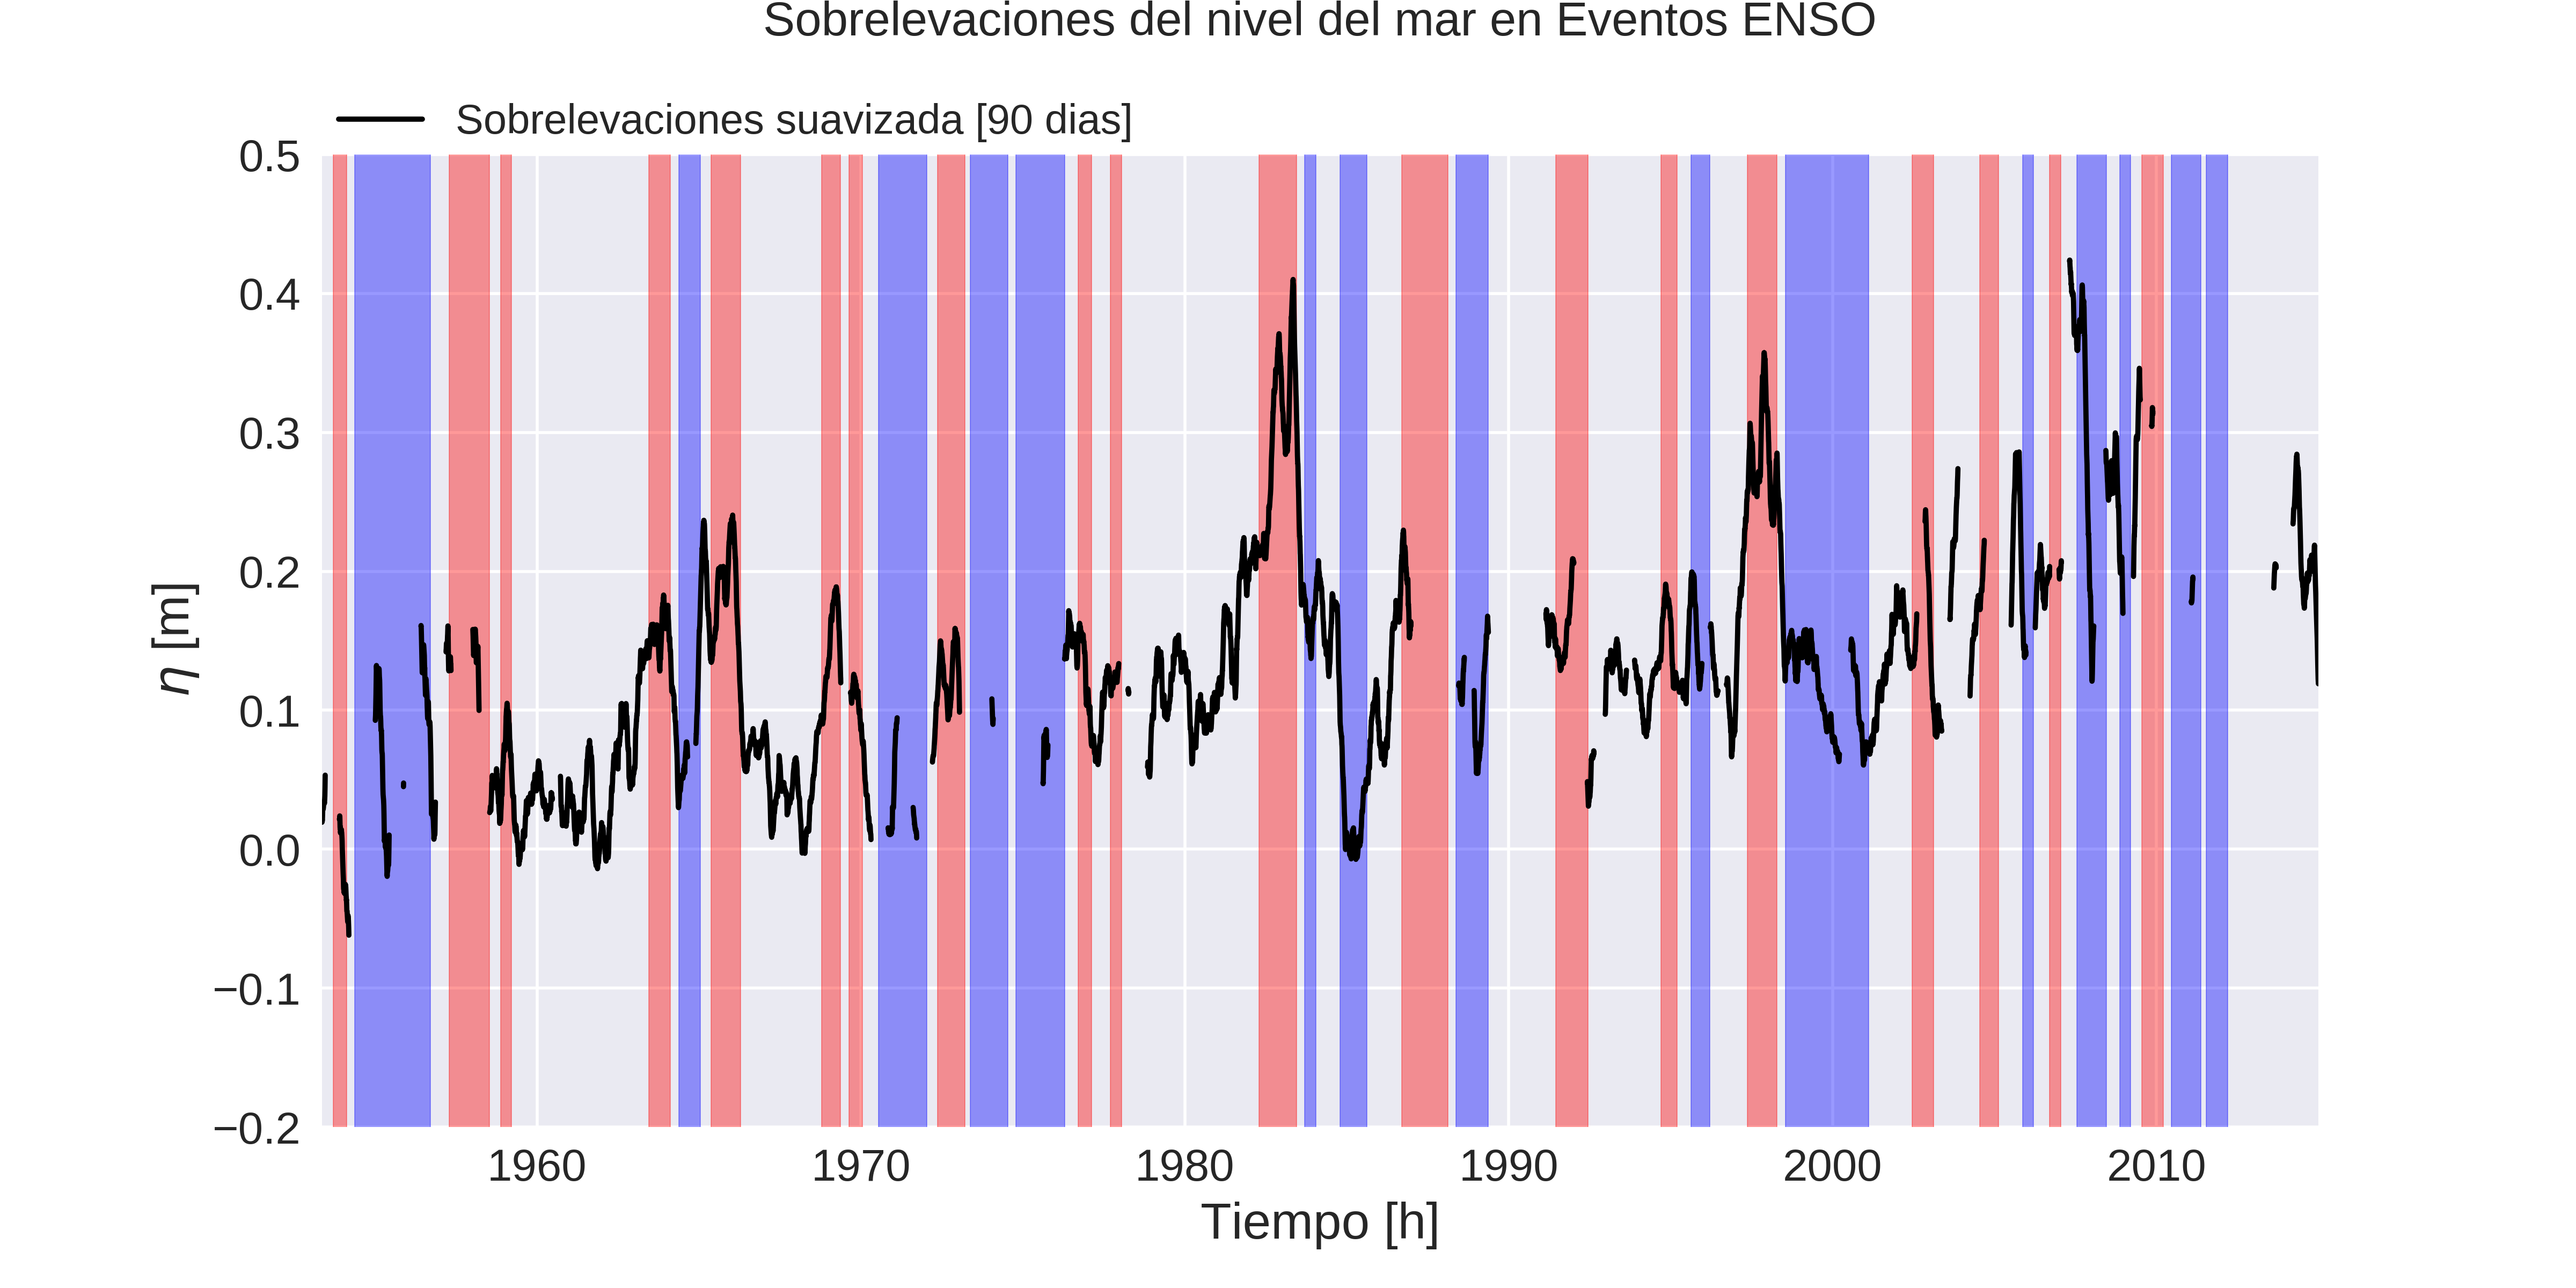
\includegraphics[width=\textwidth]{sobreelev_ENSOS.png}
	\caption{Sobrelevaciones del nivel del mar en la bahía de Buenaventura en diferentes eventos ENSOS. Las franjas rojas y azules representan fases cálidas y frías del ENSO (Eventos de Niño y Niña) }
	\label{fig:sobrelev_ENSOS}
\end{figure}






















Existen varias normas para la citaci\'{o}n bibliogr\'{a}fica. Algunas \'{a}reas del conocimiento prefieren normas espec\'{\i}ficas para citar las referencias bibliogr\'{a}ficas en el texto y escribir la lista de bibliograf\'{\i}a al final de los documentos. Esta plantilla brinda la libertad para que el autor de la tesis  o trabajo de investigaci\'{o}n utilice la norma bibliogr\'{a}fica com\'{u}n para su disciplina. Sin embargo, se solicita que la norma seleccionada se utilice con rigurosidad, sin olvidar referenciar "todos" los elementos tomados de otras fuentes (referencias bibliogr\'{a}ficas, patentes consultadas, software empleado en el manuscrito, en el tratamiento a los datos y resultados del trabajo, consultas a personas (expertos o p\'{u}blico general), entre otros).\\

\section{Ejemplos de citaciones bibliogr\'{a}ficas}
Existen algunos ejemplos para la citaci\'{o}n bibliogr\'{a}fica, por ejemplo, Microsoft Word (versiones posteriores al 2006), en el  men\'{u} de referencias, se cuenta con la opci\'{o}n de insertar citas bibliogr\'{a}ficas utilizando la norma APA (American Psychological Association) u otras normas y con la ayuda para construir autom\'{a}ticamente la lista al final del documento. De la misma manera, existen administradores bibliogr\'{a}ficos compatibles con Microsoft Word como Zotero, End Note y el Reference Manager,  disponibles a trav\'{e}s del Sistema Nacional de Bibliotecas (SINAB) de la Universidad Nacional de Colombia\footnote{Ver:www.sinab.unal.edu.co } secci\'{o}n "Recursos bibliogr\'{a}ficos" opci\'{o}n "Herramientas Bibliogr\'{a}ficas. A continuaci\'{o}n se muestra un ejemplo de una de las formas m\'{a}s usadas para las citaciones bibliogr\'{a}ficas.\\

Citaci\'{o}n individual:\cite{AG01}.\\
Citaci\'{o}n simult\'{a}nea de varios autores:
\cite{AG12,AG52,AG70,AG08a,AG09a,AG36a,AG01i}.\\

Por lo general, las referencias bibliogr\'{a}ficas correspondientes a los anteriores n\'{u}meros, se listan al final del documento en orden de aparici\'{o}n o en orden alfab\'{e}tico. Otras normas de citaci\'{o}n incluyen el apellido del autor y el a\~{n}o de la referencia, por ejemplo: 1) "...\'{e}nfasis en elementos ligados al \'{a}mbito ingenieril que se enfocan en el manejo de datos e informaci\'{o}n estructurada y que seg\'{u}n Kostoff (1997) ha atra\'{\i}do la atenci\'{o}n de investigadores dado el advenimiento de TIC...", 2) "...Dicha afirmaci\'{o}n coincide con los planteamientos de Snarch (1998), citado por Castellanos (2007), quien comenta que el manejo..." y 3) "...el futuro del sistema para argumentar los procesos de toma de decisiones y el desarrollo de ideas innovadoras (Nosella \textsl{et al}., 2008)...".\\

\section{Ejemplos de presentaci\'{o}n y citaci\'{o}n de figuras}
Las ilustraciones forman parte del contenido de los cap\'{\i}tulos. Se deben colocar en la misma p\'{a}gina en que se mencionan o en la siguiente (deben siempre mencionarse en el texto).\\

Las llamadas para explicar alg\'{u}n aspecto de la informaci\'{o}n deben hacerse con nota al pie y su nota correspondiente\footnote{Las notas van como "notas al pie". Se utilizan para explicar, comentar o hacer referencia al texto de un documento, as\'{\i} como para introducir comentarios detallados y en ocasiones para citar fuentes de informaci\'{o}n (aunque para esta opci\'{o}n es mejor seguir en detalle las normas de citaci\'{o}n bibliogr\'{a}fica seleccionadas).}. La fuente documental se debe escribir al final de la ilustraci\'{o}n o figura con los elementos de la referencia (de acuerdo con las normas seleccionadas) y no como pie de p\'{a}gina. Un ejemplo para la presentaci\'{o}n y citaci\'{o}n de figuras, se presenta a continuaci\'{o}n (citaci\'{o}n directa):\\

Por medio de las propiedades del fruto, seg\'{u}n el espesor del endocarpio, se hace una clasificaci\'{o}n de la palma de aceite en tres tipos: Dura, Ternera y Pisifera, que se ilustran en la Figura
\ref{fig:Fruto}.\\
\begin{figure}
\centering%
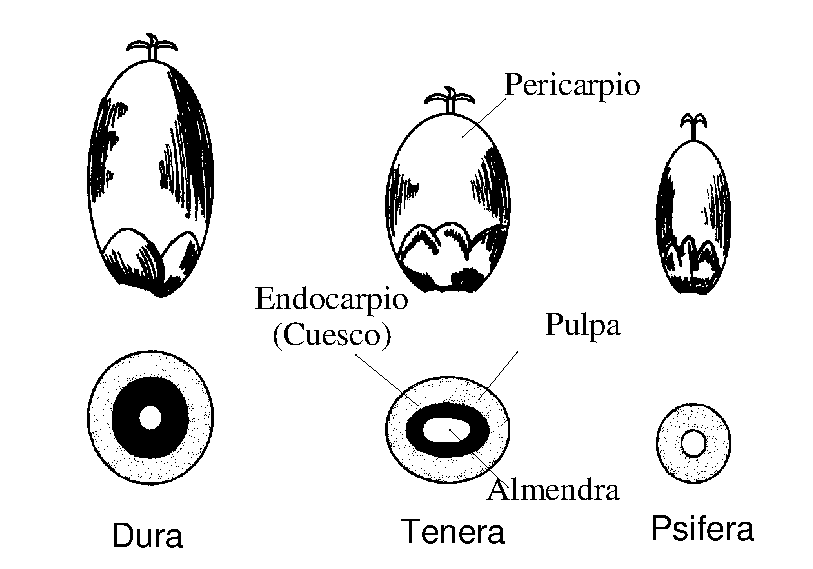
\includegraphics{Kap3/FrutoSp}%
\caption{Tipos y partes del fruto de palma de aceite \cite{AG03p,AG04p}.} \label{fig:Fruto}
\end{figure}

\section{Ejemplo de presentaci\'{o}n y citaci\'{o}n de tablas y cuadros}
Para la edici\'{o}n de tablas, cada columna debe llevar su t\'{\i}tulo; la primera palabra se debe escribir con may\'{u}scula inicial y preferiblemente sin abreviaturas. En las tablas y cuadros, los t\'{\i}tulos y datos se deben ubicar entre l\'{\i}neas horizontales y verticales cerradas (como se realiza en esta plantilla).\\

La numeraci\'{o}n de las tablas se realiza de la misma manera que las figuras o ilustraciones, a lo largo de todo el texto. Deben llevar un t\'{\i}tulo breve, que concreta el contenido de la tabla; \'{e}ste se debe escribir en la parte superior de la misma. Para la presentaci\'{o}n de cuadros, se deben seguir las indicaciones dadas para las tablas.\\

Un ejemplo para la presentaci\'{o}n y citaci\'{o}n de tablas (citaci\'{o}n indirecta), se presenta a continuaci\'{o}n:\\

De esta participaci\'{o}n aproximadamente el 60 \% proviene de biomasa
(Tabla \ref{EMundo1}).
\begin{center}
\begin{threeparttable}
\centering%
\caption{Participaci\'{o}n de las energ\'{\i}as renovables en el suministro
total de energ\'{\i}a primaria \cite{AG02i}.}\label{EMundo1}
\begin{tabular}{|l|c|c|}\hline
&\multicolumn{2}{c|}{Participaci\'{o}n en el suministro de energ\'{\i}a primaria /\% (Mtoe)\;$\tnote{1}$}\\\cline{2-3}%
\arr{Region}&Energ\'{\i}as renovables &Participaci\'{o}n de la biomasa\\\hline%
Latinoam\'{e}rica&28,9 (140)&62,4 (87,4)\\\hline%
\:Colombia&27,7 (7,6)&54,4 (4,1)\\\hline%
Alemania&3,8 (13,2)&65,8 (8,7)\\\hline%
Mundial&13,1 (1404,0)&79,4 (1114,8)\\\hline
\end{tabular}
\begin{tablenotes}
\item[1] \footnotesize{1 kg oe=10000 kcal=41,868 MJ}
\end{tablenotes}
\end{threeparttable}
\end{center}

NOTA: en el caso en que el contenido de la tabla o cuadro sea muy extenso, se puede cambiar el tama\~{n}o de la letra, siempre y cuando \'{e}sta sea visible por el lector.\\

\subsection{Consideraciones adicionales para el manejo de figuras y tablas}
Cuando una tabla, cuadro o figura ocupa m\'{a}s de una p\'{a}gina, se debe repetir su identificaci\'{o}n num\'{e}rica, seguida por la palabra continuaci\'{o}n.\\

Adicionalmente los encabezados de las columnas se deben repetir en todas las p\'{a}ginas despu\'{e}s de la primera.\\

Los anteriores lineamientos se contemplan en la presente plantilla.\\

\begin{itemize}
\item Presentaci\'{o}n y citaci\'{o}n de ecuaciones.
\end{itemize}

La citaci\'{o}n de ecuaciones, en caso que se presenten, debe hacerse como lo sugiere esta plantilla. Todas las ecuaciones deben estar numeradas y citadas detro del texto.\\

Para el manejo de cifras se debe seleccionar la norma seg\'{u}n el \'{a}rea de conocimiento de la tesis  o trabajo de investigaci\'{o}n.\\
\chapter{Cap\'{\i}tulo 3}
Se deben incluir tantos cap\'{\i}tulos como se requieran; sin embargo, se recomienda que la tesis  o trabajo de investigaci\'{o}n tenga un m\'{\i}nimo 3 cap\'{\i}tulos y m\'{a}ximo de 6 cap\'{\i}tulos (incluyendo las conclusiones).\\
\chapter{Objetivos}
Conocer el efecto del ENSO en la variabilidad interanual del nivel del mar en la zona costera de Buenaventura.

\section{Objetivos específicos}

\begin{itemize}
	\item Identificar la relación del nivel del mar en Buenaventura con las fases cálidas y frías del ENSO a través del índice ONI.
	\item Caracterizar los eventos Niño y Niña en términos de su duración y amplitud así como desde el comportamiento del nivel del mar en Buenaventura.
	\item Analizar espectralmente la serie mensual de nivel del mar para la información del mareógrafo y filtrarla en la banda de interés (2-6 años)
	\item Conocer la variabilidad espacial del nivel del mar en el Pacífico Tropical a través de mapas de varianza y funciones ortogonales empíricas.
	\item Caracterizar espacialmente el nivel del mar durante la ocurrencia de eventos Niño y Niña.
	\item Determinar una región costera frente a la bahía de Buenaventura a partir de la información espacial y su respectiva serie de nivel del mar promediada espacialmente
	\item Elegir zonas de mayor correlación rezagada entre el nivel del mar, temperatura, corrientes zonales, corrientes meridionales y el nivel del mar en la costa.
	\item Predecir la variación interanual del nivel del mar en la costa a partir del uso de una red neuronal artificial
\end{itemize}
\chapter{Conclusiones y recomendaciones}
\section{Conclusiones}

El ENSO es el fenómeno más importante en la variabilidad interanual del nivel del mar en la bahía de Buenaventura y durante sus fases cálidas se presentan sobrelevaciones de hasta 35 cm sobre el nivel medio del mar y descensos de hasta 40 cm. El comportamiento del nivel del mar puede variar entre eventos niño y niña y es función de la duración dela fase cálida o fría, la intensidad del evento. El promedio de las sobrelevaciones ocurridas en los meses niño es de 43.3 cm y el promedio de los descensos durante los meses niña es de 45.2 cm. El promedio de las duraciones de los eventos ENSO es menor al promedio de las duraciones de los eventos Niña, esto puede verse explicado porque las fases frías del ENSO son más estables que las cálidas \cite{Gouirand2003}.

El ENSO puede aportar hasta 10 cm a la sobrelevación del nivel del mar, cómo aparece en ciertos registros en el evento Niño de 1982-1983, e incluso, es posible que ciertas condiciones amplifiquen o no estas sobrelevaciones, convirtiéndose en una amenaza para las comunidades costeras. Las sobrelevaciones y descensos del nivel del mar debidos solamente a fenómeno ENSO actúan en conjunto con la climatología anual del nivel y otras condiciones específicas que pueden intensificar y/o sostener dichos aumentos/descensos.

El patrón espacio-temporal más importante del nivel del mar en la escala interanual en el Pacífico Tropical es el ENSO y la varianza asociada a la banda espectral en la que se estudia puede representar hasta el 50\% de la varianza total del nivel del mar en regiones cercanas al trópico

Las aumentos persistentes e intensos del nivel del mar durante los eventos Niño logran atravesar el Pacífico de Oeste a Este y modificar las condiciones de nivel del mar en las costas de Suramérica y en determinadas ocasiones, generar posteriores descensos del nivel del mar.

Es posible la implementación de herramientas de pronóstico de los aportes del ENSO al nivel del mar en la bahía de Buenaventura con una red neuronal artificial construida y entrenada que predice el 30\% de los datos (conjunto de datos de validación) con un RMSE de 0.01 m y una correlación de Spearman igual a 0.83. Su estructura se resume en: 2 variables de entrada, nivel del mar y velocidad longitudinal de las corrientes, 2 nodos en una capa intermedia oculta y una capa de salida, las caracerísticas de su configuració son una función de activación tangente hiperbólica y el uso de corrección del sesgo.


\section{Recomendaciones}

Futuras investigaciones pueden involucrar el estudio y la correlación del nivel del mar con el principal forzador de la superficie libre del océano, el viento. Es posible que se determinen zonas con correlaciones rezagadas altas y suficientes para determinar una serie predictora determinante para el entrenamiento de la RNA, inclusive, puede buscarse información con registros temporales más extensos para calibrar mejor la red durante la etapa de entrenamiento y obtener mejores rendimientos durante la etapa de validación

Conocido el aporte del ENSO al nivel del mar en Buenaventura, quedan interrogantes acerca de las condiciones previas que deben existir tanto para que dichos aumentos y/o descensos se amplifiquen o sean más duraderos, como para que tengan efectos menores en la costa. 

El estudio anterior puede ampliarse a otras regiones del Pacifico colombiano como el municipio de Tumaco, Nariño, dónde también se han registrado aumentos súbitos del nivel mar. El modelo aplicado se debería mejorar para realizar una herramienta tecnológica que ayude a tomar decisiones rápidas para la gestión del riesgo en la costa.
\begin{appendix}
\chapter{Anexo: Nombrar el anexo A de acuerdo con su contenido}\label{AnexoA}
Los Anexos son documentos o elementos que complementan el cuerpo de la tesis o trabajo de investigaci\'{o}n y que se relacionan, directa o indirectamente, con la investigaci\'{o}n, tales como acetatos, cd, normas, etc.\\

\chapter{Anexo: Nombrar el anexo B de acuerdo con su contenido}
A final del documento es opcional incluir \'{\i}ndices o glosarios. \'{E}stos son listas detalladas y especializadas de los t\'{e}rminos, nombres, autores, temas, etc., que aparecen en el mismo. Sirven para facilitar su localizaci\'{o}n en el texto. Los \'{\i}ndices pueden ser alfab\'{e}ticos, cronol\'{o}gicos, num\'{e}ricos, anal\'{\i}ticos, entre otros. Luego de cada palabra, t\'{e}rmino, etc., se pone coma y el n\'{u}mero de la p\'{a}gina donde aparece esta informaci\'{o}n.\\

\chapter{Anexo: Nombrar el anexo C de acuerdo con su contenido}
MANEJO DE LA BIBLIOGRAF\'{I}A: la bibliograf\'{\i}a es la relaci\'{o}n de las fuentes documentales consultadas por el investigador para sustentar sus trabajos. Su inclusi\'{o}n es obligatoria en todo trabajo de investigaci\'{o}n. Cada referencia bibliogr\'{a}fica se inicia contra el margen izquierdo.\\

La NTC 5613 establece los requisitos para la presentaci\'{o}n de referencias bibliogr\'{a}ficas citas y notas de pie de p\'{a}gina. Sin embargo, se tiene la libertad de usar cualquier norma bibliogr\'{a}fica de acuerdo con lo acostumbrado por cada disciplina del conocimiento. En esta medida es necesario que la norma seleccionada se aplique con rigurosidad.\\

Es necesario tener en cuenta que la norma ISO 690:1987 (en Espa\~{n}a, UNE 50-104-94) es el marco internacional que da las pautas m\'{\i}nimas para las citas bibliogr\'{a}ficas de documentos impresos y publicados. A continuaci\'{o}n se lista algunas instituciones que brindan par\'{a}metros para el manejo de las referencias bibliogr\'{a}ficas:\\

\begin{center}
\centering%
\begin{tabular}{|p {7.5 cm}|p {7.5 cm}|}\hline
\arr{Instituci\'{o}n}&Disciplina de aplicaci\'{o}n\\\hline%
Modern Language Association (MLA)&Literatura, artes y humanidades\\\hline%
American Psychological Association (APA)&Ambito de la salud (psicolog\'{\i}a, medicina) y en general en todas las ciencias sociales\\\hline
Universidad de Chicago/Turabian &Periodismo, historia y humanidades.\\\hline
AMA (Asociaci\'{o}n M\'{e}dica de los Estados Unidos)&Ambito de la salud (psicolog\'{\i}a, medicina)\\\hline
Vancouver &Todas las disciplinas\\\hline
Council of Science Editors (CSE)&En la actualidad abarca diversas ciencias\\\hline
National Library of Medicine (NLM) (Biblioteca Nacional de Medicina)&En el \'{a}mbito m\'{e}dico y, por extensi\'{o}n, en ciencias.\\\hline
Harvard System of Referencing Guide &Todas las disciplinas\\\hline
JabRef y KBibTeX &Todas las disciplinas\\\hline
\end{tabular}
\end{center}

Para incluir las referencias dentro del texto y realizar lista de la bibliograf\'{\i}a en la respectiva secci\'{o}n, puede utilizar las herramientas que Latex suministra o, revisar el instructivo desarrollado por el Sistema de Bibliotecas de la Universidad Nacional de Colombia\footnote{Ver: www.sinab.unal.edu.co}, disponible en la secci\'{o}n "Servicios", opci\'{o}n "Tr\'{a}mites" y enlace "Entrega de tesis".

\end{appendix}
\addcontentsline{toc}{chapter}{\numberline{}Bibliograf\'{\i}a}
\bibliographystyle{plaindin_esp}
\bibliography{BibliMSc}
\end{document}